\subsection{Zero Moment Point}
\label{sec::311_zmp}
The key metric in this work, for the generation of a dynamically balanced gait, is the zero moment point. The concept was first introduced by Miomir Vukobratovi\'{c} and Davor Juri\v{c}i\'{c} in 1968 \cite{vukobratovic1968contribution}\cite{vukobratovic1969contribution} and first utilized 1984 to generate walking trajectories for the WL-10RD robot \cite{yamaguchi1993development}. The most intuitive understanding for the ZMP arises by thinking about the realization of the simplest arbitrary possible walking motion for which a humanoid robot will not fall. This motion is achieved by ensuring the feet's whole area, and not only the edge, is in contact with the ground \cite{vukobratovic2004zero}, or put in other words, we require the robot not to rotate about its feet edges. This constraint can be met by having a reaction force $\bm{F}_r$ between the foot and the ground, which compensates for all external moments $\bm{M}_x$, and $\bm{M}_y$ around the x-, and y-axis at any time (fig. \ref{fig::311_zmp}).
\begin{figure}[h]
	\centering
	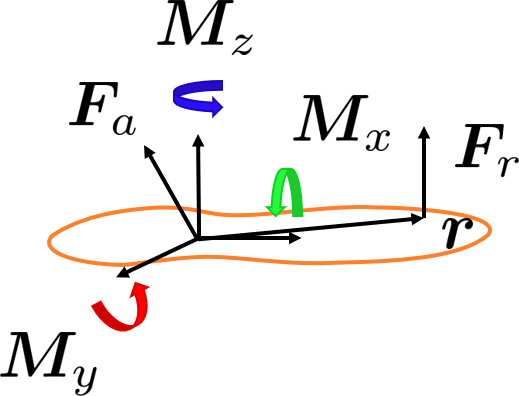
\includegraphics[scale=.5]{chapters/03_background/img/zero_moment_point.png}
	\caption{Forces acting on the sole.}
	\label{fig::311_zmp}
\end{figure}
The point $\bm{r}$, at which the reaction force acts, is physically only meaningful if it lies within the support polygon of the foot. Not only can it not exist outside of the support polygon, since there was no point of interaction between the foot and the ground then, but also was the robot to overturn under these circumstances. Therefore, the ZMP is defined as that point on the ground at which the net moment of the inertial forces has no component along the horizontal axes \cite{hirai1998development}\cite{dasgupta1999making}. We now came to appreciate the importance of the support polygon for the definition of the zero moment point. 
\begin{figure}[h]
	\centering
	
\includegraphics[scale=.5]{chapters/03_background/img/support_polygon.png}
	\caption{Full support polygon, and the resulting support polygon with security margin (dashed lines).}
	\label{fig::311_support_polygon}
\end{figure}
The support polygon is defined as the convex hull of all contact points of the feet with the ground, so the minimal number of points to fully contain all of them. As the most restrictive case for balance, in this work we will only consider the support polygon of one foot at a time. Since the convex hull of a foot is well described by a rectangle, we only rely on the foot width (\href{https://github.com/mhubii/nmpc_pattern_generator/blob/bc79a6d4f9bcfd3794146355af44429f5b7a9fe0/libs/pattern_generator/configs.yaml#L14}{link}), and foot length (\href{https://github.com/mhubii/nmpc_pattern_generator/blob/bc79a6d4f9bcfd3794146355af44429f5b7a9fe0/libs/pattern_generator/configs.yaml#L15}{link}) to fully describe it. Also, to ensure that the zero moment point never comes close to the edges of the feet and therefore to provide balance, we define a security margin to their boarders (\href{https://github.com/mhubii/nmpc_pattern_generator/blob/bc79a6d4f9bcfd3794146355af44429f5b7a9fe0/libs/pattern_generator/configs.yaml#L3}{link}). The respective values are robot specific and can be set in the configurations file by following the provided links.
\\\\
As already pointed out, within this work, we will use a simplified physical model of the humanoid solve the optimal control problem in real time. We will deal with this approximation in the following paragraph - Zero Moment Point of a Linear Inverted Pendulum.
\subsubsection{Zero Moment Point of a Linear Inverted Pendulum}
Dynamically balanced walking trajectories can be generated by simplifying the dynamics of humanoid robots to those of a linear inverted pendulum \cite{kajita2003biped}. A rigorous derivation for the analytic relation between the center of mass and the zero moment point of a linear inverted pendulum can be found in \cite{kajita2014introduction}, but for the sake of simplicity we rather explain the physics in terms of cutting forces, for which a short introduction can be found in the summary of the lecture Robotics 1 (\href{https://drive.google.com/file/d/1aN1ujXTOlHzO2kLPK7TQRkWfdY-pGzUF/view}{link}). 
\begin{figure}[h]
	\centering
	\subcaptionbox{}%
	[.4\linewidth]{
\includegraphics[scale=.3]{chapters/03_background/img/inverted_pendulum.png}}
	\subcaptionbox{}%
	[.4\linewidth]{
\includegraphics[scale=.3]{chapters/03_background/img/inverted_pendulum_free_body_diagram.png}}
	\caption{Linear inverted pendulum with a support polygon (a), and the corresponding free body diagram with cutting forces $\bm{S}_{x/y/z}$ (b).}
	\label{fig::311_lip}
\end{figure}
The system of interest is shorty depicted in figure \ref{fig::311_lip}. We assume the support polygon of the shown linear inverted pendulum to have zero mass. By introducing cutting forces $\bm{S}_{x/y/z}$ for each degree of freedom in which the motion of the linear inverted pendulum is restricted, we obtain the free body diagram (fig. \ref{fig::311_lip}), for which the acting forces are
\begin{align}
	m\ddot{\bm{c}} &=\quad\bm{S} - \bm{F}_g 
	\label{eq::311_pendulum_force} \\
	\bm{0} &= -\bm{S}+\bm{F}_r
	\label{eq::311_support_polygon_force}
\end{align}
where $\bm{S}=\bm{S}_x+\bm{S}_y+\bm{S}_z$. The respective moments, since we do not take any inertias into account, are given by
\begin{align}
	\bm{0} &= (\bm{0}-\bm{c})\times\bm{S} + \bm{M} 
	\label{eq::311_pendulum_moment}\\	
	\bm{0} &= (\bm{r}-\bm{0})\times\bm{F}_r - \bm{M}
	\label{eq::311_support_polygon_moment}	
\end{align}
where the transfer of the moment $\bm{M}$ may for example be induced by friction. If we replace $\bm{S}=\bm{F}_r$ from eq. \ref{eq::311_support_polygon_force}, equations \ref{eq::311_pendulum_moment} and \ref{eq::311_support_polygon_moment} yield 
\begin{align}
	\bm{0} = (\bm{r}-\bm{c})\times\bm{S} = \begin{pmatrix}
	\quad(r_y - c_y)S_z - (r_z - c_z)S_y \\
	-(r_x - c_x)S_z + (r_z - c_z)S_x \\
	\quad(r_x - c_x)S_y - (r_y - c_y)S_x
	\end{pmatrix}
	\label{eq::311_momentum_transfer}
\end{align}
Since our goal is to have a robot that does not fall, we want to achieve that the acceleration along the z-axis becomes zero, hence $\ddot{c}_z=0$. Given this assumption, we can infer from eq. \ref{eq::311_pendulum_force} that $S_z=mg$, as well as $S_x = \ddot{c}_xm$, and $S_y = \ddot{c}_ym$. Furthermore, our foot shall not lift off the floor, and therefore we have $r_z=0$. If we take these assumptions and plug them into the first to rows of eq. \ref{eq::311_momentum_transfer}, we find
\begin{align}
	r_x &= c_x - c_z\frac{\ddot{c}_x}{g}\\
	r_y &= c_y - c_z\frac{\ddot{c}_y}{g}
	\label{eq::311_zmp}
\end{align}
Therein, $r_x$, and $r_y$ are the x-, and y-coordinates of the zero moment point, given the assumption of a linear inverted pendulum. We can see that the position if dependent on the height of the point mass, which is in turn dependent on the robot. The specific values can be set in the configurations file (\href{https://github.com/mhubii/nmpc_pattern_generator/blob/bc79a6d4f9bcfd3794146355af44429f5b7a9fe0/libs/pattern_generator/configs.yaml#L27}{link}).
\\\\
We have now found a simple analytic expression for the relationship of the zero moment point and the center of mass, which will help us to formulate an optimal control problem that we can solve in real time. This simplification is of course only true to some extend, and we need to find a way to verify its accuracy. The easiest way to do so is to measure the real zero moment point. We will further elaborate on this within the next paragraph - Measurement of the Zero Moment Point, and we will derive a method that only relies on force torque sensors in the ankle.
\subsubsection{Measurement of the Zero Moment Point}
There are several methods that enable us to measure the position of the zero moment point, among them the utilization of pressure sensitive soles, as outlined in \cite{kajita2014introduction}. Furthermore, there exist approximate approaches that involve the knowledge of all acting external forces \cite{huang2001planning}, which can for example be obtained from unconstrained inverse dynamics \cite{michel2017dynamic}. Since we can rely on measurements of force torque sensors that are located at the ankles, we will infer the position of the zero moment point from them \cite{kajita2014introduction}. If we consider the force torque sensor to be located a position $\bm{p}_i$ (fig. \ref{fig::311_force_torque}), then we can obtain the moment about any point $\bm{p}$ according to eq. \ref{eq::311_moment}.
\begin{align}
	\bm{\tau}(\bm{p}) = (\bm{p}_i-\bm{p})\times \bm{f}_i + \bm{\tau}_i
	\label{eq::311_moment}
\end{align}
by definition, the moment about the zero moment point vanishes along the horizontal axes, therefore we can then set $\tau_x = \tau_y = 0$ in eq. \ref{eq::311_moment} and then solve for the position to obtain the zero moment point (eq. \ref{eq::311_x_pos_zmp} and \ref{eq::311_y_pos_zmp}).
\begin{align}
	p_x &= \frac{\left[-\tau_{i,y}-(p_{i,z}-p_z)f_{i,x}+p_{i,x}f_{i,z}\right]}{f_{i,z}}
	\label{eq::311_x_pos_zmp}\\
	p_y &= \frac{\left[-\tau_{i,x}-(p_{i,z}-p_z)f_{i,y}+p_{i,y}f_{i,z}\right]}{f_{i,z}}
	\label{eq::311_y_pos_zmp}
\end{align}
If we further choose our coordinate system to lie along the z-axis of the force torque sensor, we can simplify equations \ref{eq::311_x_pos_zmp} and \ref{eq::311_y_pos_zmp} 